\documentclass[12pt]{article}

\usepackage{booktabs}% http://ctan.org/pkg/booktabs
\usepackage[utf8]{inputenc}
\usepackage{changepage}
\usepackage{pgfplots}
\usepackage{amssymb}
\usepackage{xcolor}
\usepackage{hyperref}
\usepackage{listings}
\usepackage[T1]{fontenc}
\usepackage[utf8]{inputenc}
\usepackage{adjustbox}
\usepackage{amsmath}
\usepackage{mathtools}
\usepackage{biblatex}
\lstset{
  language=Python,
  numbers=left,
  numberstyle=\tiny,
  stepnumber=1,
  numbersep=5pt,
  tabsize=4,
  basicstyle=\ttfamily,
  columns=fullflexible,
  keepspaces,
}
\hypersetup{
    colorlinks,
    citecolor=black,
    filecolor=black,
    linkcolor=black,
    urlcolor=black
}

% Set page size and margins
% Replace `letterpaper' with `a4paper' for UK/EU standard size
\usepackage[letterpaper,top=2cm,bottom=2cm,left=3cm,right=3cm,marginparwidth=1.75cm]{geometry}

% Useful packages
\usepackage{amsmath}
\usepackage{mathtools}
\usepackage{graphicx}
\newenvironment{para}{\begin{adjustwidth}{13mm}{}}{\end{adjustwidth}}

\newcommand\tab[1][1cm]{\hspace*{#1}}

\newcommand{\tabitem}{\llap{\textbullet}}
\newcommand{\Hsquare}{%
\text{\fboxsep=-.2pt\fbox{\rule{0pt}{1ex}\rule{1ex}{0pt}}}%
}

\newtheorem{Definizione}{Definizione}[subsection]
\newtheorem{Lemma}{Lemma}[subsection]
\newtheorem{Teorema/Definizione}{Teorema/Definizione}[subsection]
\newtheorem{Corollario}{Corollario}[subsection]
\newtheorem{Teorema}{Teorema}[subsection]
\newtheorem{Proposizione}{Proposizione}[subsection]
\newtheorem{Notazione}{Notazione}[subsection]
\newtheorem{Commento}{Commento}[subsection]
\newtheorem{Dimostrazione}{Dimostrazione}[subsection]
\newtheorem{Osservazione}{Osservazione}[subsection]
\newtheorem{Nota}{Nota}[subsection]

\title{Ricerca operativa e pianificazione delle risorse}
\author{spitfire}
\date{A.A. 2023-2024}
\begin{document}
\begin{figure}
    \centering
    
\includegraphics[width=0.35\textwidth]{Images/Logo scienze bicocca.png}
\end{figure}

\vspace{10cm}
\date{A.A. 2024-2025}


\maketitle

\newpage

\tableofcontents
\newpage

\section{Prerequisiti di Algebra Lineare}
\subsection{Matrici e vettori}
Una matrice è una tabella contenente numeri.
Se la tabella è costituita da $m$ righe e $n$ colonne si parla
di una matrice  $m \times n$. 
Una matrice viene detta \textbf{matrice quadrata} se il numero di righe
e colonne coincidono. \newline
Una matrice $1 \times m$ viene detto \textbf{vettore riga m-dimensionale} \newline
Una matrice $m \times 1$ viene detto \textbf{vettore colonna m-dimensionale}. \newline
La notazione maggiormente utilizzata per indicare una matrice è
$$A = [a_{ij}]$$
Con $a_{ij}$ elemento generico della i-esima riga e j-esima colonna della matrice $A$.
Se $A = [a_{ij}]$ è una matrice $m \times n$, la matrice $n \times m$
$$A^T=[a_{ij}]$$
viene detta \textbf{matrice trasposta} della matrice $A$.

Se $A = [a_{ik}]$ è una matrice $m \times p$ e $B = [b_{kj}]$ è una matrice $p \times n$ la loro
\textbf{matrice prodotto} è $m \times n$ e definita come:
$$A \cdot B = C = [c_{ij}] \; con \; c_{ij} = \sum_{k = 1}^{p} a_{ik} \cdot b_{kj}$$
Date due matrici $m \times n, A = [a_{ij}]$ e $B = [b_{ij}]$, la loro \textbf{matrice somma} è definita come segue:
$$A+B=C=[c_{ij}] \; con \; c_{ij} = a_{ij} + b_{ij}$$
La \textbf{moltiplicazione} di una \textbf{matrice A per una costante $\alpha$} fornisce come risultato quanto segue:
$$\alpha \cdot A = [\alpha \cdot a_{ij}]$$
Questa moltiplicazione è \textbf{commutativa}. \newline
Siano $v_1, v_2, ..., v_n$ n vettori, riga o colonna; essi vengono detti
\textbf{linearmente indipendenti} tra loro se, prendendo $n$ coefficienti $a_1, a_2, ..., a_n$ la seguente uguaglianza
$$a_1 \cdot v_1 + a_2 \cdot v_2 + ... + a_n \cdot v_n = 0$$
risulta verificata solo se $a_1 = a_2 = ... = a_n = 0$. \newline
Al contrario, se esistono coefficienti $a_1, a_2, ..., a_n$ non tutti nulli per cui
$$a_1 \cdot v_1 + a_2 \cdot v_2 + ... + a_n \cdot v_n = 0$$
i vettori $v_1, v_2, ..., v_n$ sono detti \textbf{linearmente dipendenti}. \newline
Un insieme di $n$ vettori ad $n$ dimensioni linearmente indipendenti costituisce una \textbf{base per uno spazio a n dimensioni}.
Se un insieme di vettori $v_1, v_2, ..., v_n$ costituisce una base per uno spazio ad $n$ dimensioni, allora ogni vettore $x$ che appartiene
a quello spazio è \textbf{combinazione lineare dei vettori della base}. \newline
Una matrice quadrata $m \times m$ si dice \textbf{matrice singolare} se l'insieme degli $m$ vettori riga (o colonna), ottenuti considerando
ogni riga (o colonna) come un vettore, è \textbf{linearmente dipendenti}.
Se, viceversa, l'insieme degli $m$ vettori è linearmente indipendente, la matrice si dice \textbf{matrice non singolare}. \newline
Una matrice quadrata $A = [a_{ij}]$ con $a_{ij} = 0$ per ogni $i \neq j$ viene detta \textbf{matrice diagonale}. \newline
La matrice diagonale $A = [a_{ij}]$, con $a_{ii} = 1$ per ogni $i$ viene detta \textbf{matrice identità}, solitamente indicata con $I$.
Se $A$ NON è una matrice singolare, allora esiste una matrice $A^{-1}$ detta \textbf{matrice inversa} della matrice $A$, tale per cui vale la
seguente relazione di uguaglianza:
$$A \cdot A^{-1} = A^{-1} \cdot A = I$$
Il \textbf{determinante} di una matrice quadrata $A$ si indica con $det(A)$ ed è un numero (esiste solo per matrici quadrate), nel caso
specifico di una matrice $2 \times 2$ si definisce come segue:
$$det(A) = det\begin{pmatrix}
    a_{11} & a_{12} \\
    a_{21} & a_{22}
\end{pmatrix} = a_{11} \cdot a_{22} - a_{12} \cdot a_{21}$$
Il determinante di una matrice quadrata $A$ $m \times m$ si ottiene utilizzando la seguente regola ricorsiva, detta \textbf{formula di Laplace}:
Se $A_{ij}$ è la matrice $(m-1) \times (m-1)$, ottenuta togliendo la i-esima riga e la j-esima colonna di A, il determinante di A risulta:
$$det(A) = \sum_{j=1}^{m} (-1)^{i+j} \cdot a_{ij} \cdot det(A_{ij}) \; (formula \; per \; righe)$$
$$det(A) = \sum_{i=1}^{m} (-1)^{i+j} \cdot a_{ij} \cdot det(A_{ij}) \; (formula \; per \; colonne)$$
Se la matrice è singolare, allora $det(A) = 0$. \newline
Una matrice quadrata $A$ ammette inversa se e solo se non è singolare.
\subsection{Equazioni lineari}
Un' \textbf{equazione lineare} nelle variabili $x_1, x_2, ..., x_n$ è un'equazione nella seguente forma:
$$a_1 \cdot x_1 + a_2 \cdot x_2 + ... + a_n \cdot x_n = b$$
dove $a_1, a_2, ..., a_n$ e $b$ sono delle costanti.
Si dice \textbf{soluzione dell'equazione} un qualsiasi vettore $|y_1, y_2, ..., y_n| \in \mathbb{R}^n$ tale che:
$$a_1 \cdot y_1 + a_2 \cdot y_2 + ... + a_n \cdot y_n = b$$
Un \textbf{sistema di m equazioni lineari in n variabili} è definito come segue:
$$\begin{cases}
    a_{11} \cdot x_1 + a_{12} \cdot x_2 + ... + a_{1n} \cdot x_n = b_1 \\
    a_{21} \cdot x_1 + a_{22} \cdot x_2 + ... + a_{2n} \cdot x_n = b_2 \\
    ... \\
    a_{m1} \cdot x_1 + a_{m2} \cdot x_2 + ... + a_{mn} \cdot x_n = b_m
\end{cases}$$
dove $a_{ij}$ e $b_{j}$, $i = 1,...,n$; $j = 1,...,m$ sono costanti.
Una \textbf{soluzione del sistema lineare} è un qualsiasi vettore $|y_1, y_2, ..., y_n| \in \mathbb{R}^n$ tale che le $m$ equazioni
del sistema lineare siano contemporaneamente soddisfatte.
Trovare le soluzioni del sistema lineare equivale a individuare il punto di intersezione tra le sue equazioni, ammesso che un tale punto esista. \newline
Un sistema di equazioni lineari può essere:
\begin{itemize}
    \item \textbf{Consistente}: se ammette almeno una soluzione, in caso contrario viene detto \textbf{inconsistente}
    \item \textbf{Determinato}: se costituito da un numero di equazioni uguale al numero di incognite $m = n$. Un tale sistema ha \textbf{una sola soluzione}
    \item \textbf{Sovradeterminato}: se costituito da più equazione che incognite $m>n$. Un tale sistema è spesso, ma non sempre, inconsistente
    \item \textbf{Sottodeterminato}: se costituito da meno equazioni che incognite $m<n$. Un tale sistema ammette infinite soluzioni
\end{itemize}
Consideriamo la forma matriciale del sistema costituito da $m$ equazioni lineari in $n$ incognite
$$A \cdot x = b$$
dove
\begin{itemize}
    \item $A$ è una matrice $m \times n$ (nota)
    \item $x$ è un vettore colonna in $n$ dimensioni (incognito)
    \item $b$ è un vettore colonna in $m$ dimensioni (noto)
\end{itemize}
Si definisce \textbf{rango della matrice A} come segue:
\begin{itemize}
    \item \textbf{Rango di riga}: numero massimo di righe linearmente indipendenti
    \item \textbf{Rango di colonna}: numero massimo di colonne linearmente indipendenti
\end{itemize}
Se $rango \; di \; riga = rango \; di \; colonna$ allora $rk(A) \leq min(m, n)$ \newline
Se $rk(A) = min (m, n)$, allora la matrice A viene detta \textbf{a rango pieno}. \newline
Data la matrice dei coefficienti $A$, si dice \textbf{matrice aumentata} la matrice $C = A,b$ ottenuta
dalla matrice $A$ aggiungendo come colonna aggiuntiva il vettore dei termini noti $b$.
Avremo quanto segue:
\begin{itemize}
    \item $rk(C) > rk(A)$: Il sistema lineare non ammette soluzione
    \item $rk(C) = rk(A)$: il sistema lineare ammette soluzione
\end{itemize}
Assumiamo $rk(C) = rk(A)$, allora:
\begin{itemize}
    \item Caso $m \geq n$
    \begin{itemize}
        \item Se $rk(A) = n$, allora il sistema ha una soluzione unica
        \item Se $rk(A) < n$, allora il sistema ha infinite soluzioni
    \end{itemize}
    \item Caso $m < n$
    \begin{itemize}
        \item Se $rk(A) \leq m$, allora il sistema ha infinite soluzioni
    \end{itemize}
\end{itemize}
Come si risolve un sistema di equazioni lineari? Abbiamo due metodi:
\subsubsection{Metodo di eliminazione}
Procediamo come segue:
\begin{enumerate}
    \item Selezionare una variabile, e risolvere una delle equazioni rispetto ad essa e eliminare
    la variabile in questione dalle altre equazioni
    \item Tralasciare l'equazione utilizzata nel passo di eliminazione e tornare al passo 1)
    \item Applicare il processo di \textbf{Back-walk substitution}: dall'ultima equazione, tornare indietro e risolvere le restanti
\end{enumerate}
\subsubsection{Metodo di eliminazione di Gauss}
Il metodo di eliminazione di Gauss è un metodo di eliminazione che utilizza solo le operazioni elementari su matrici, cioé:
\begin{itemize}
    \item Moltiplicare una riga per uno scalare non nullo
    \item Sommare una riga moltiplicata per uno scalare non nullo con un'altra riga
    \item Permutare le righe 
\end{itemize}
\begin{Teorema}
    Applicare operazioni elementari a un sistema di equazioni lineari non cambia l'insieme delle sue soluzioni.
\end{Teorema}
\section{Prerequisiti di Analisi Matematica}
\subsection{Funzioni di una variabile}
Si dice \textbf{funzione} una terna $(A, B, f)$ con:
\begin{itemize}
    \item $A, B$ due insiemi non vuoti
    \item $f$ una legge che ad ogni elemento $x \in A$ associa uno ed uno solo elemento $f(x) \in B$
\end{itemize}
dove:
\begin{itemize}
    \item $A$ è detto dominio della funzione $f$, anche indicato con $dom(f)$
    \item $B$ è detto codominio della funzione $f$
    \item Scriviamo $f: A \rightarrow B$ e $x \in dom(f) \rightarrow f(x)$, per indicare la legge che alla variabile indipendente $x$ associa la sua immagine $f(x)$
\end{itemize}
Data una funzione $f: A \rightarrow B$, se esiste, finito o meno, il limite:
$$\lim_{h \rightarrow 0} \frac{f(x_0 + h) - f(x_0)}{h} = \frac{f(x) - f(x_0)}{x - x_0}$$
esso viene chiamato \textbf{derivata della funzione f nel punto $x_0$} e viene indicato con
$$f'(x_0) = \frac{d}{dx}f(x_0)$$
Se $f'(x_0) \in \mathbb{R}$, allora $f$ si dice derivabile in $x_0$. \newline
\newpage
Riportiamo le derivate elementari:
\begin{itemize}
    \item Se $f(x) = c, \forall x \in \mathbb{R}$ allora $f'(x) = 0, \forall x \in \mathbb{R}$
    \item Se $f(x) = x^n, n \in \mathbb{N}, n \geq 2$ allora $f'(x) = n \cdot x^{n-1}, \forall x \in \mathbb{R}$
    \item Se $f(x) = \frac{1}{x}, \forall x \in \mathbb{R}^+$ allora $f'(x) = -\frac{1}{x^2}, \forall x \in \mathbb{R}^+$
    \item Se $f(x) = log(x), x \in \mathbb{R}^+$ allora $f'(x) = \frac{1}{x}, \forall x \in \mathbb{R}^+$
\end{itemize}
Data una funzione $f: \mathbb{R} \rightarrow \mathbb{R}$ e un punto $x_0 \in \mathbb{R}$, allora
\begin{itemize}
    \item $f$ derivabile in $x_0 \Rightarrow f$ continua in $x_0$
    \item $f$ continua in $x_0 \not\Rightarrow f$ derivabile in $x_0$
\end{itemize}
Se $f, g: \mathbb{R} \rightarrow \mathbb{R}$ sono derivabili in $x_0 \in \mathbb{R}$, allora
\begin{itemize}
    \item $\forall c \in \mathbb{R}$, la funzione $c \cdot f$ è derivabile in $x_0$ e $(c \cdot f)'(x_0) = c \cdot f'(x_0)$
    \item La funzione $f + g$ è derivabile in $x_0$ e $(f+g)'(x_0) = f'(x_0) + g'(x_0)$
\end{itemize}
Se $f, g: \mathbb{R} \rightarrow \mathbb{R}$ sono derivabili in $x_0 \in \mathbb{R}$, allora anche la funzione $f \cdot g$ è derivabile
in $x_0$ e si ha quanto segue
$$(f \cdot g)'(x_0) = f'(x_0) \cdot g(x_0) + f(x_0) \cdot g'(x_0)$$
Date due funzioni $f, g: \mathbb{R} \rightarrow \mathbb{R}$, con $f$ derivabile in $x_0 \in \mathbb{R}$ e $g$ derivabile in
$f(x_0)$, allora $g \circ f$ è derivabile in $x_0$ e si ha quanto segue:
$$(g \circ f)'(x_0) = g'(f(x_0)) \cdot f'(x_0)$$
La derivata della \textbf{derivata prima $f'$} in $x_0 \in \mathbb{R}$ viene detta \textbf{derivata seconda} e indicata come $f''(x_0)$. \newline
La derivata è il \textbf{coefficiente angolare} della retta tangente alla funzione nel punto di derivazione $x_0$. \newline
Data una funzione $f(x)$ definita su un intervallo chiuso $[a,b]$ diremo che la funzione è:
\begin{itemize}
    \item \textbf{Crescente}: nell'intervallo $[a,b]$ quando per ogni coppia di punti $x_1, x_2 \in [a,b]$ con $x_1 < x_2$ risulta che $f(x_1) < f(x_2)$
    \item \textbf{Decrescente}: nell'intervallo $[a,b]$ quando per ogni coppia di punti $x_1, x_2 \in [a,b]$ con $x_1 < x_2$ risulta che $f(x_1) > f(x_2)$
\end{itemize}
Per determinare se la funzione $f:[a,b] \rightarrow \mathbb{R}$ sia crescente o decrescente in un punto $x_0 \in [a,b]$ è possibile ricorrere alla valutazione della sua derivata
nel punto $x_0$, infatti:
\begin{itemize}
    \item Se $f'(x_0) >0$ allora è crescente nel punto considerato $x_0$
    \item Se $f'(x_0) <0$ allora la funzione è decrescente nel punto considerato $x_0$
\end{itemize}
Una funzione $f:[a,b] -> \mathbb{R}$ si dice \textbf{convessa} se $\forall x_1, x_2 \in [a,b]$ con $x_1 < x_2$ vale la seguente relazione
$$f(x) \leq f(x_1) + \frac{f(x_2) - f(x_1)}{x_2 - x_1} \cdot (x - x_1) \; \forall x \in [a,b]$$
\textbf{strettamente convessa} se:
$$f(x) < f(x_1) + \frac{f(x_2) - f(x_1)}{x_2 - x_1} \cdot (x - x_1) \; \forall x \in [a,b]$$
Una funzione $f:[a,b] -> \mathbb{R}$ si dice \textbf{concava} se $\forall x_1, x_2 \in [a,b]$ con $x_1 < x_2$ vale la seguente relazione
$$f(x) \geq f(x_1) + \frac{f(x_2) - f(x_1)}{x_2 - x_1} \cdot (x - x_1) \; \forall x \in [a,b]$$
\textbf{strettamente concava} se:
$$f(x) > f(x_1) + \frac{f(x_2) - f(x_1)}{x_2 - x_1} \cdot (x - x_1) \; \forall x \in [a,b]$$
Data una funzione continua $f:[a,b] \rightarrow \mathbb{R}$ possiamo affermare che
\begin{itemize}
    \item Essa è crescente (decrescente) in un punto $x \in [a,b]$ se la sua derivata prima è positiva (negativa) in $x$
    \item I \textbf{punti di stazionarietà} (estremanti) della funzione sono i punti in cui la derivata prima della funzione $f$ si annulla cambiando di segno,
    nello specifico si ha un punto di \textbf{massimo} in $x \in [a,b]$ quando $f'$ passa da un valore \textbf{positivo} a un valore \textbf{negativo}, mentre si ha un punto di
    \textbf{minimo} in $x \in [a,b]$ quando $f'$ passa da un valore $negativo$ a un valore $positivo$
    \item È detta \textbf{lineare} se la sua \textbf{derivata prima è una funzione costante}
\end{itemize}
\begin{center}
    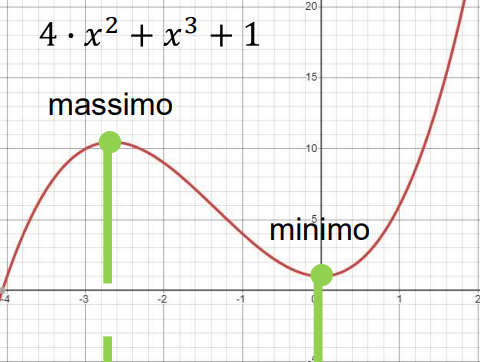
\includegraphics[width = 0.50\textwidth]{Images/1.PNG}
\end{center}
Data una funzione continua $f:[a,b] \rightarrow \mathbb{R}$ e un punto $x_0 \in [a,b]$, si dice che $f$ ha un minimo o massimo locale (o relativo) nel punto 
$x_0$ quando esiste un intorno $l(x_0)$ nel quale risulta
\begin{itemize}
    \item $f(x) \geq f(x_0) \forall x \in l(x_0)$ allora $x_0$ è un \textbf{minimo locale}
    \item $f(x) \leq f(x_0) \forall x \in l(x_0)$ allora $x_0$ è un \textbf{massimo locale}
    \item $x_0$ è un \textbf{minimo locale relativo} se la funzione è decrescente immediatamente a sinistra di $x_0$ e crescente immediatamente a destra
    \item $x_0$ è un \textbf{massimo locale relativo} se la funzione è crescente immediatamente a sinistra di $x_0$ e decrescente immediatamente a destra 
\end{itemize}
Il punto minimo (massimo) locale in cui la funzione $f$ assume il valore minimo (massimo) viene detto \textbf{minimo} (\textbf{massimo}) \textbf{globale} o \textbf{assoluto}.
\subsection{Funzioni in due o più variabili}
Una funzione continua definita come $f: \mathbb{R} \times \mathbb{R} \rightarrow \mathbb{R}$ che associa ad ogni coppia di numeri reali $(x_1, x_2) \in \mathbb{R} \times \mathbb{R} = R^2$ uno
e un solo valore $y \in \mathbb{R}$ viene detta \textbf{funzioni in due variabili} $(x_1, x_2)$, che vengono dette \textbf{variabili indipendenti}, mentre la variabile $y$ viene riferita con il termine di
\textbf{variabile dipendente}.
Questo concetto è generalizzabile al caso in cui si considerino $n$ variabili indipendenti $(x_1, x_2, ..., x_n) \in \mathbb{R}^n$. In questo caso
si parla di funzione $f: \mathbb{R}^n \rightarrow \mathbb{R}$ in $n$ variabili indipendenti, funzione che descrive una "regola" per ottenere dall'insieme delle $n$ variabili indipendenti $(x_1, x_2, ..., x_n)$ un singolo
valore reale di $y$. \newline
Una funzione in $n$ variabili $f: \mathbb{R}^n \rightarrow \mathbb{R}$ viene detta \textbf{funzione lineare} nelle variabili $(x_1, x_2, ..., x_n)$ se è nella forma:
$$f(x_1, x_2, ..., x_n) = a_0 + a_1 \cdot x_1 + a_2 \cdot x_2 + ... + a_n \cdot x_n$$
dove $a_0, a_1, ..., a_n$ sono parametri che assumono valore reale. \newline
Una funzione in $n$ variabili $f: \mathbb{R}^n \rightarrow \mathbb{R}$ viene detta \textbf{funzione quadratica} nelle variabili $(x_1, x_2, ..., x_n)$ se è nella forma:
$$f(x_1, x_2, ..., x_n) = a_0 + \sum_{k=1}^n b_k \cdot x_k + \sum_{i = 1}^n \sum_{j \neq i,1}^n h_{ij} \cdot x_i \cdot x_j + \sum_{k=1}^n h_{kk} \cdot x_k^2$$
\begin{center}
    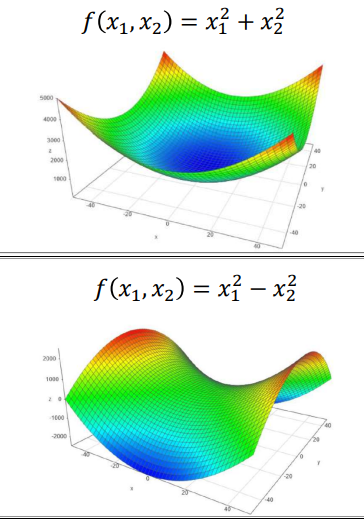
\includegraphics[width = 0.35\textwidth]{Images/2.PNG}
\end{center}
Le \textbf{curve di livello} di una funzione $f: \mathbb{R}^n \rightarrow \mathbb{R}$ sono ottenute disegnando i punti
$(x_1, x_2, ..., x_n)$ in cui la funzione ha valore constante $k$, vale a dire tutti i punti $(x_1, x_2, ..., x_n) \in \mathbb{R}^n$ per i quali vale la seguente uguaglianza
$$f(x_1, x_2, ..., x_n) = k$$
\begin{center}
    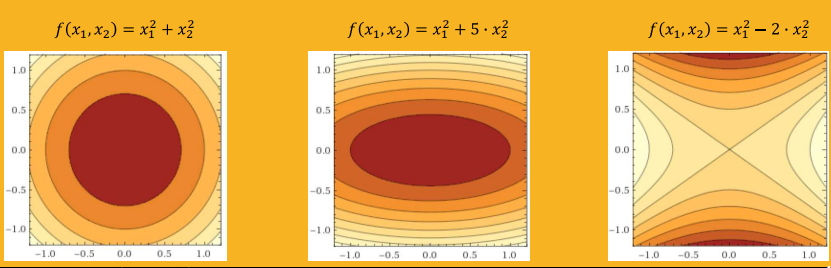
\includegraphics[width = 1\textwidth]{Images/3.PNG}
\end{center}
Dal punto di vista geometrico, le linee di livello sono le \textbf{proiezioni ortogonali} sul piano $Oxy$ delle curve ottenute
intersecando il piano $z=k$ e il grafico della funzione $z = f(x_1, x_2, ..., x_n)$
\begin{center}
    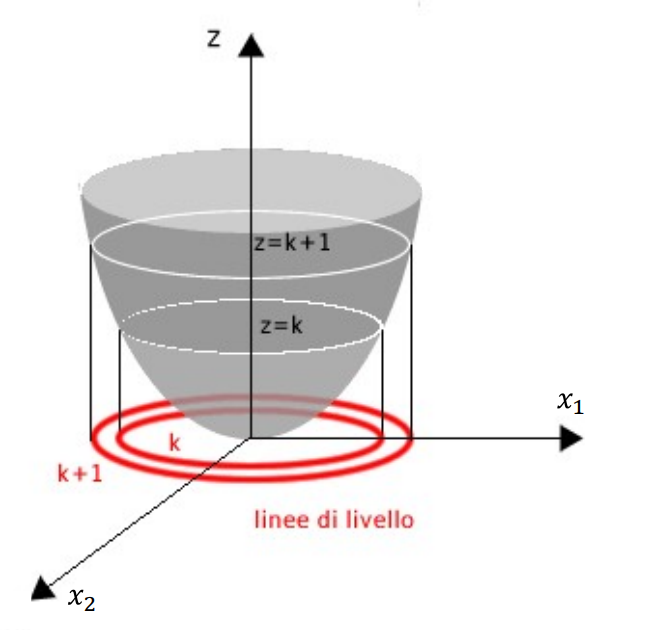
\includegraphics[width = 0.50\textwidth]{Images/4.PNG}
\end{center}
Data la funzione in 2 variabili $f: \mathbb{R}^2 \rightarrow \mathbb{R}$:
\begin{itemize}
    \item Si dice \textbf{derivata parziale rispetto a $x_1$} la seguente funzione:
    $$\frac{\partial f(x_1, x_2)}{\partial x_1} = f_{x_1} = f'_{x_1}$$
    Essa rappresenta il tasso con cui varia la funzione $f(x_1, x_2)$ al variare della variabile $x_1$, quando sia fissato e mantenuto costante
    il valore della variabile $x_2$.
    \item Si dice \textbf{derivata parziale rispetto a $x_2$} la seguente funzione:
    $$\frac{\partial f(x_1, x_2)}{\partial x_2} = f_{x_2} = f'_{x_2}$$
    Essa rappresenta il tasso con cui varia la funzione $f(x_1, x_2)$ al variare della variabile $x_2$, quando sia fissato e mantenuto costante
    il valore della variabile $x_1$
    \item Si dice \textbf{gradiente} il vettore i cui coefficienti sono le derivate parziali della funzione $f(x_1, x_2)$ rispetto alle variabili $x_1$ e $x_2$, esso è denotato nel seguente modo:
    $$\nabla f(x_1, x_2) = \begin{pmatrix}
        \frac{\partial f(x_1, x_2)}{\partial x_1} \\
        \frac{\partial f(x_1, x_2)}{\partial x_2}
    \end{pmatrix} = \begin{pmatrix}
        f'_{x_1} \\
        f'_{x_2}
    \end{pmatrix}$$
\end{itemize}
Data la funzione in 2 variabili $f: \mathbb{R}^2 \rightarrow \mathbb{R}, f(x_1, x_2)$:
\begin{itemize}
    \item Si dice \textbf{derivata parziale seconda rispetto a $x_1$} e $x_1$ la seguente funzione:
    $$\frac{\partial}{\partial x_1} \frac{\partial f(x_1, x_2)}{\partial x_1} = f_{x_1, x_1} = f'_{x_1, x_1}$$
    \item Si dice \textbf{derivata parziale seconda rispetto a $x_1$} e $x_2$ la seguente funzione:
    $$\frac{\partial}{\partial x_1} \frac{\partial f(x_1, x_2)}{\partial x_2} = f_{x_1, x_2} = f'_{x_1, x_2}$$
    \item Si dice \textbf{derivata parziale seconda rispetto a $x_2$} e $x_1$ la seguente funzione:
    $$\frac{\partial}{\partial x_2} \frac{\partial f(x_1, x_2)}{\partial x_1} = f_{x_2, x_1} = f'_{x_2, x_1}$$
    \item Si dice \textbf{derivata parziale seconda rispetto a $x_2$} e $x_2$ la seguente funzione:
    $$\frac{\partial}{\partial x_2} \frac{\partial f(x_1, x_2)}{\partial x_2} = f_{x_2, x_2} = f'_{x_2, x_2}$$
\end{itemize}
In particolare:
$$\frac{\partial}{\partial x_1} \frac{\partial f(x_1, x_2)}{\partial x_2} = f_{x_1, x_2} = f'_{x_1, x_2} = \frac{\partial}{\partial x_2} \frac{\partial f(x_1, x_2)}{\partial x_1} = f_{x_2, x_1} = f'_{x_2, x_1}$$
Data la funzione in 2 variabili $f: \mathbb{R}^2 \rightarrow \mathbb{R}, f(x_1, x_2)$, si dice
\textbf{matrice Hessiana} la matrice quadrata delle derivate parziali:
$$H = \begin{pmatrix}
    f_{x_1, x_1} & f(x_1, x_2) \\
    f_{x_2, x_1} & f(x_2, x_2)
\end{pmatrix}$$
\textbf{Condizione necessaria del primo ordine}: Data la funzione in 2 variabili $f: \mathbb{R}^2 \rightarrow \mathbb{R}, f(x_1, x_2)$, un punto
$(x_1, x_2)$ può essere un punto critico (minimo, massimo o sella) solo se il suo gradiente nel punto $(x_1, x_2)$ è nullo:
$$\nabla f(x_1, x_2) = \begin{pmatrix}
    0 \\
    0
\end{pmatrix}$$
Non ne conosciamo però la natura! (Minimo? Massimo? Sella?) \newpage
\textbf{Condizioni sufficienti del secondo ordine}:
Supponiamo che $(x_1, x_2)$ sia un punto critico di $f(x_1, x_2)$. Calcoliamo il determinante della matrice Hessiana:
$$det(H) = f_{x_1,x_1} (x_1, x_2) \cdot f_{x_2 x_2}(x_1, x_2) - (f_{x_1, x_2}(x_1, x_2))^2$$
Abbiamo i seguenti casi:
\begin{itemize}
    \item $det(H) > 0$:
    \begin{itemize}
        \item $f_{x_1, x_1} > 0 \Rightarrow (x_1, x_2)$ è un minimo relativo di $f(x_1, x_2)$
        \item $f_{x_1, x_1} < 0 \Rightarrow (x_1, x_2)$ è un massimo relativo di $f(x_1, x_2)$
    \end{itemize}
    \item $det(H) < 0 \Rightarrow (x_1, x_2)$ è un punto di sella di $f(x_1, x_2)$
\end{itemize}
Data la funzione in 2 variabili $f: \mathbb{R}^2 \rightarrow \mathbb{R}, f(x_1, x_2)$, se la sua matrice Hessiana $H$ è tale per cui
$f_{x_1, x_1} > 0$ e $det(H) > 0$ allora la funzione è \textbf{convessa}. Se la funzione è  convessa, allora ogni punto di minimo e di massimo sono
\textbf{globali} poiché ammette solamente un punto dove il gradiente si annulla
\section{Modelli nella Ricerca Operativa}


\end{document}